\documentclass{article}

\usepackage[margin=1.25in]{geometry}
\usepackage{graphicx}
\usepackage[hidelinks]{hyperref}

\begin{document}

\title{Mysterious House Guide}
\date{}
\maketitle

\section*{Introduction}
This is a complete guide to the Amazon Alexa skill: Mysterious House. 
The game consists of three floors each containing some puzzle to solve. 
There are three alternate endings available at the end of floor 3, two negative endings and one secret positive ending. To report bugs and give feedback on the game or this guide you can find contact details on the Mysterious House website: \url{www.mysterioushouse.co.uk}

\section*{Floor 1}
To progress past the first floor you have to get down the ladder.
Larry won't let you down the ladder without permission from Barry and Barry won't give you permission.
To progress you have to lie.

\begin{figure}[htb]
	\centering
	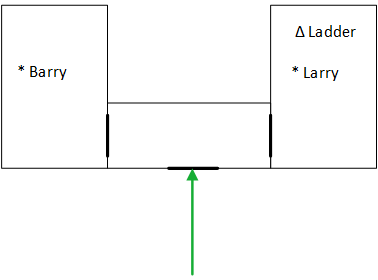
\includegraphics{Floor1.png}
\end{figure}

Steps to complete this floor:

\begin{enumerate}
	\item Go to the right room and talk to Larry, he will tell you to get permission from Barry.
	\item Go out of the room and head to the left room, talk to Barry who will refuse to let you get downstairs.
	\item Return back to the left room and talk to Larry, he will ask you if Barry said yes.
	\item Lie to Larry and say \textit{yes}, Larry will let you down to floor 2.
\end{enumerate}

\section*{Floor 2}
Floor 2 is a maze. By specifying local directions: forward, backward, left and right, you have to navigate from a starting position to the ladder.
As directions are local, turning left four times will cause you to walk in a circle.
A haunted suit of armour enemy patrols around the maze, if you walk to a junction at the same time as the enemy then you are knocked out and forced restart the floor from the start.
To give a hint to any player who wishes to work out the puzzle on their own, a map of the maze is shown below alongside the enemy patrol route.

\begin{figure}[htb]
	\centering
	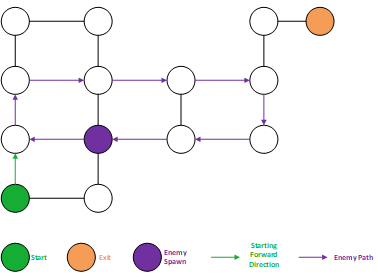
\includegraphics[width=4.5in]{Floor2-Map.png}
\end{figure}

There are multiple ways of reaching the exit, all direct routes will bump into the suit of armour so some indirection is required. Here is one of the solutions for the maze (starting at the start position and facing North):

\begin{enumerate}
	\item Go Right
	\item Follow around to the Left
	\item Turn Left
	\item Turn Right at the split
	\item Turn Right at the next junction
	\item Continue Forward through the next junction
	\item Continue Forward again at the next junction
	\item Turn left at the split
	\item Follow the path around to the right
	\item You have reached the exit
\end{enumerate}

\newpage
Here is a map of that solution:

\begin{figure}[htb]
	\centering
	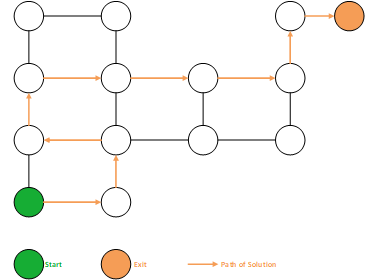
\includegraphics[width=4.5in]{Floor2-Solution.png}
\end{figure}

\section*{Floor 3}
Floor 3 is the final floor of Mysterious House, here you are presented with two foods: sugared doughnuts and a Victoria sponge cake, and asked to choose.
If you pick the sugared doughnuts, you will be poisoned and Larry will appear, he will fade away and you will wake up having taken the place of Larry in the mysterious house.
If you pick the cake, you will be poisoned and the haunted suit of armour will appear, the spirit will fade away and you will wake up having taken the place of the haunted suit of armour.
These are two alternate negative endings of the game, there is a secret good ending however.

\subsection*{Secret Ending}
The secret good ending can be triggered by saying \textit{both} to the choice between the cake and the doughnuts.
(If you want to try that ending, do it now as I'm about to spoil what happens).
This time Barry will appear laughing, revealing he had been behind all of this and had planned to enslave you, the poisons in the two foods cancel each other out leaving you unharmed, being unable to stop you any further you leave Barry and the Mysterious House alive.

\end{document}